\chapter{Methods}

\section{Traditional Computer Vision-based Approach}

This section is related to all the experiments done on the traditional computer 
vision-based approach. The general scheme of the driver's attention model is 
shown in Figure \ref{fig:driver_attention}. 
The model is divided into four main stages: data synchronization, homography 
projection of the gaze, scene perception, and the driver's behavioral model. 

The data synchronization stage is responsible for aligning the data from the 
different sensors. In particular it is important that gaze data and 
images from the 
eye-tracking glasses are well synchronized each other and with video frames 
from the camera installed on the roof top of the car.

The homography projection of the gaze stage is responsible for projecting the 
gaze of the driver from the ETG camera plane to the roof top camera plane.
In this way we have a wider, more stable and accurate representation of 
the outside environment.
It is possible to 
estimate the homography transformation making the approximation that the matched 
keypoints are far away enough from the vehicle. This is a reasonable 
approximation since the driver is usually looking at the road and the objects 
far away from the vehicle. Moreover, the baseline of the stereo vision system is 
small compared to the depth of the keypoints.
The optimal way to estimate the projection would be through the epipolar 
geometry, estimating the fundamental matrix and the essential matrix. 
However, we have an uncalibrated stereo setup, and the baseline between the two 
cameras is not fixed. Even though it could be possible to integrate GPS data 
to estimate the two matrices, there is a consistent noise error that affects 
accuracy of the estimation.
The homography estimation is then divided in three steps: detection of keypoints 
in the two images through the SIFT algorithm, matching of the keypoints through 
RANSAC, and estimation of the homography matrix through the least squares method.

The scene perception stage is responsible for detecting and tracking the vulnerable 
users in the scene, such as pedestrians and cyclists. The detection is done 
through the YOLOv8 algorithm and the tracking through ByteTrack. In this way 
it is possible to compare the gaze of the driver with the state of the targets, 
including their position.

Finally, on the top, there is the driver's attention model. The responsibility 
of this block is to classify dangerous scenarios given the data from the 
driver and the scene. However, this block is sensitive to the quality of the 
signals of the previous stages.

\begin{figure}
    \centering
    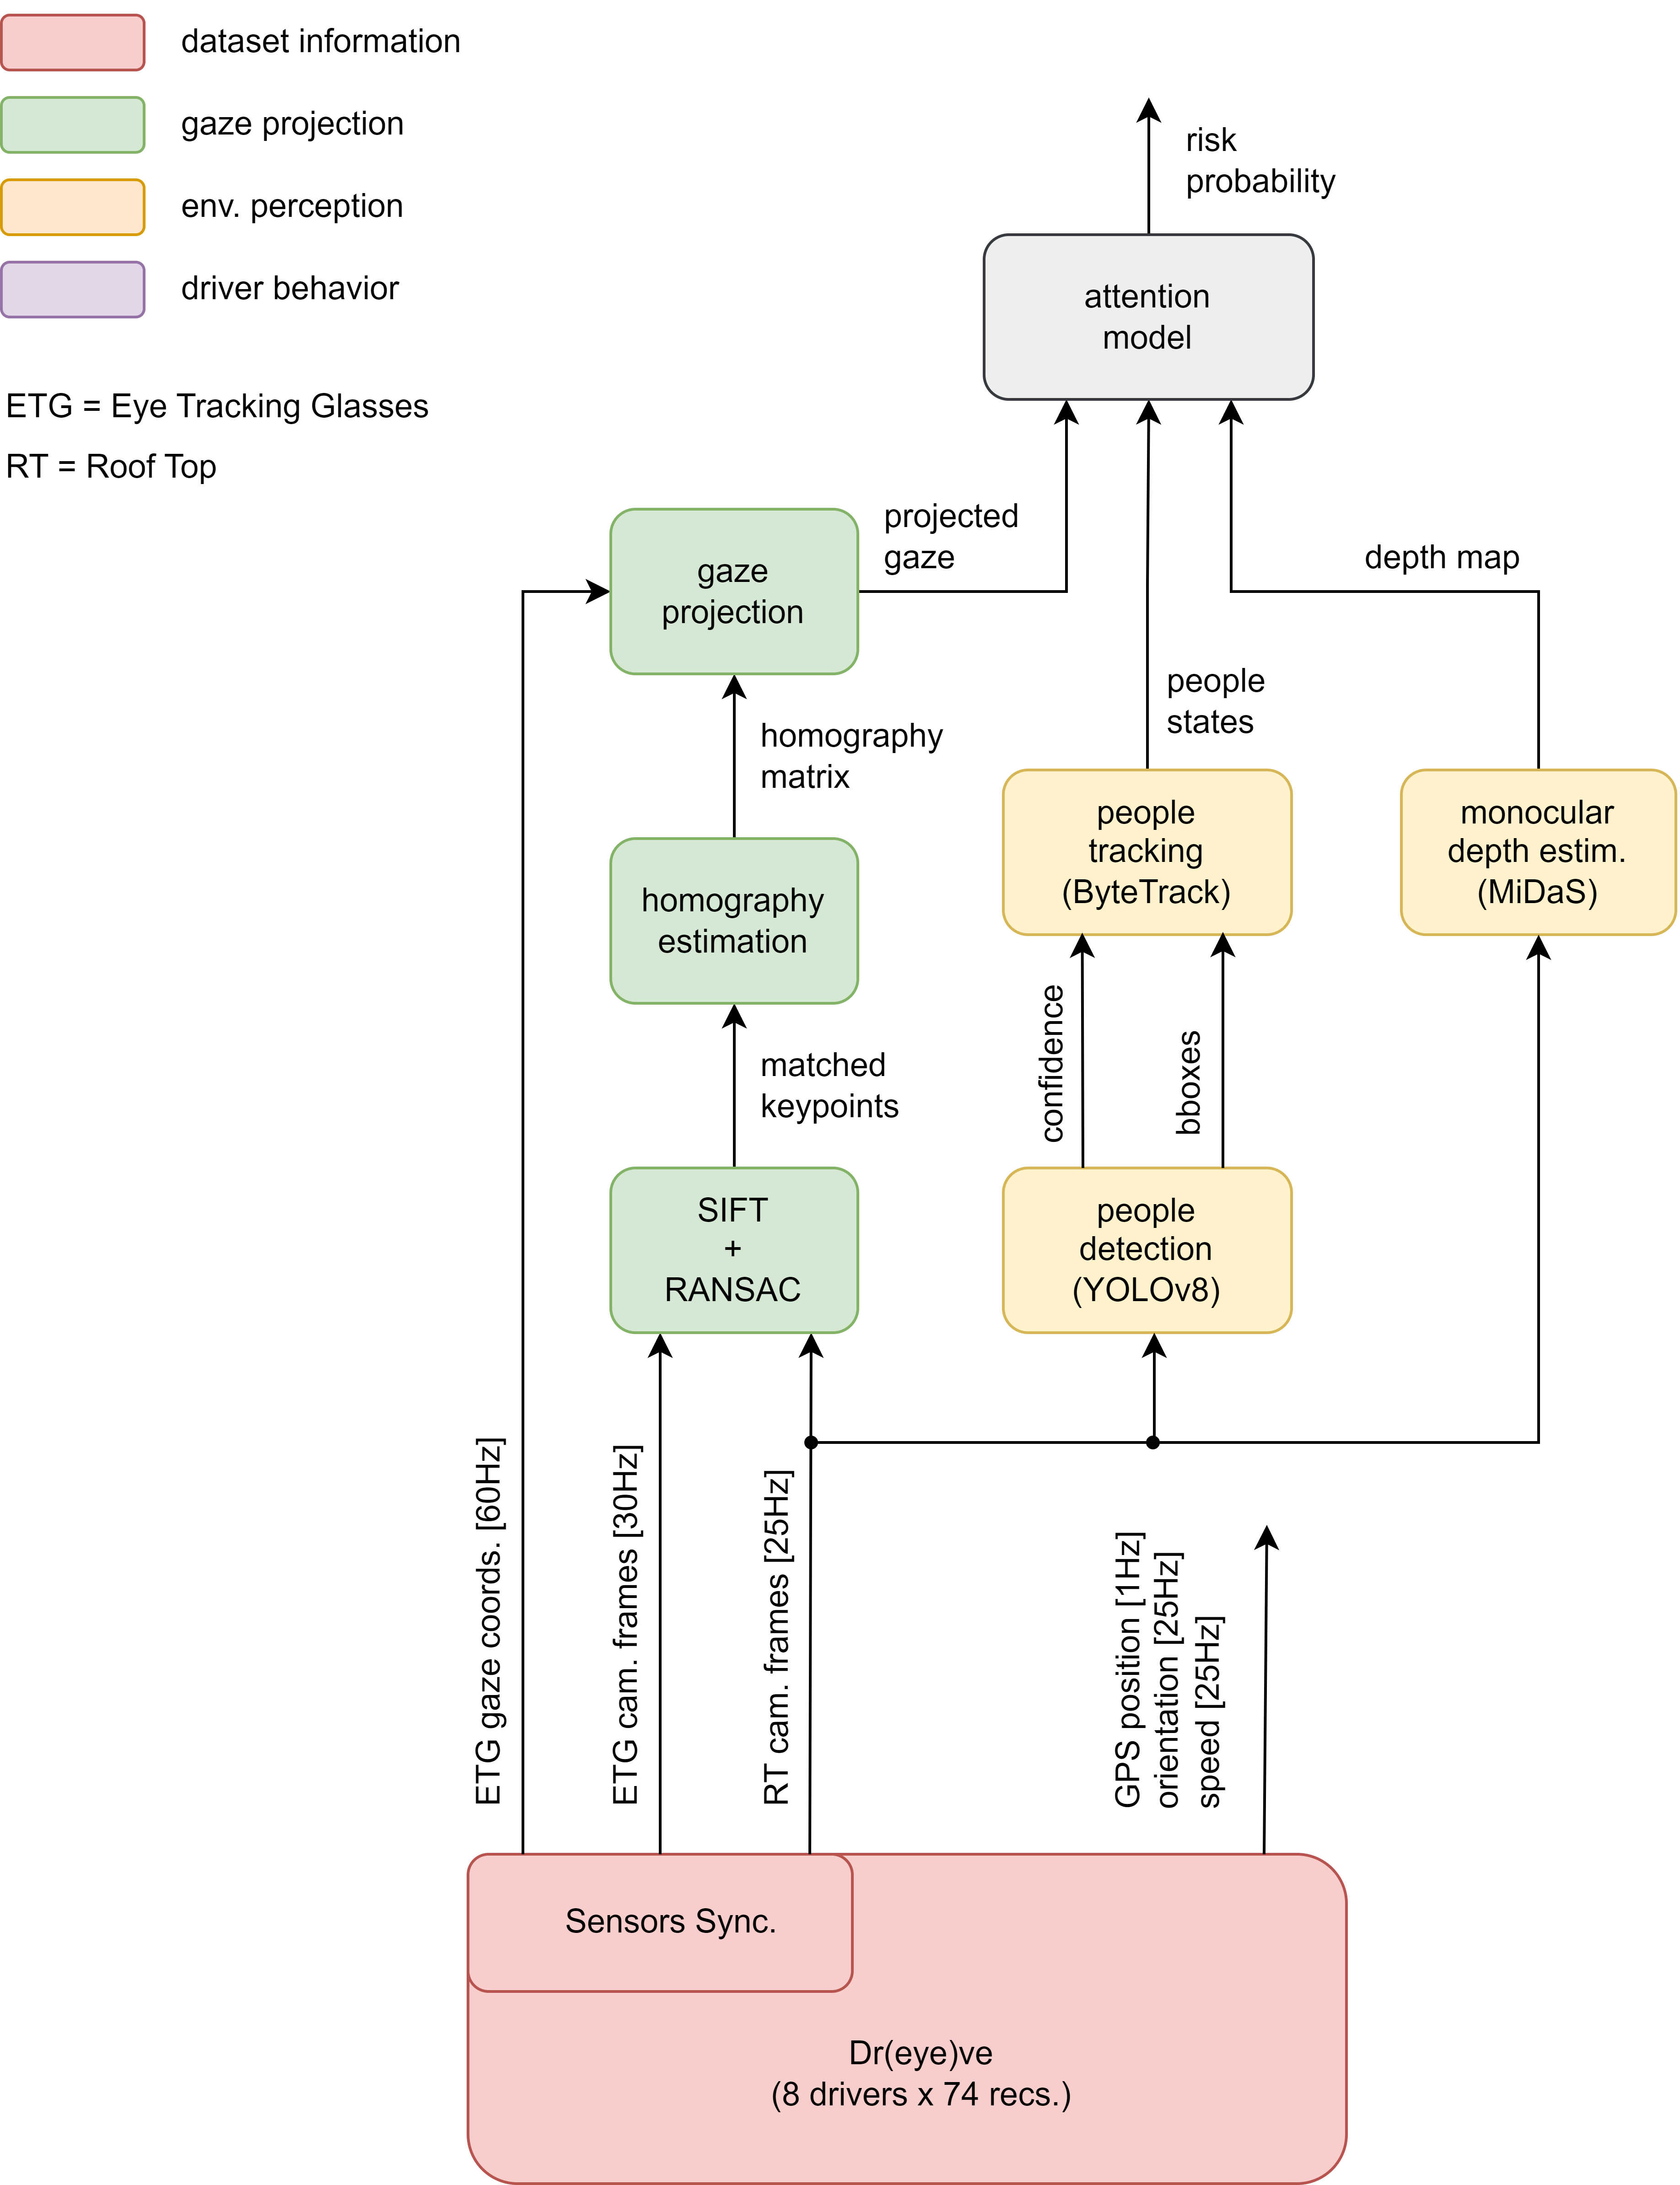
\includegraphics[width=0.9\textwidth]{images/dreyeve/classic_scheme.png}
    \vspace*{0.6cm}
    \caption[Traditional computer vision-based driver's attention model]
    {The overall driver's attention scheme. It is divided into four main 
    stages: data synchronization, homography projection of the gaze, scene 
    perception and the driver's behavioral model.
    }
    \label{fig:driver_attention}
\end{figure}

\subsection{Homography Data Structure}
The Dr(eye)ve dataset is composed of 74 sequences of five minutes each. 
Moreover, the two cameras are not synchronized. 
The ETG camera has a frame rate of 30 fps, while the roof top camera has a 
frame rate of 25 fps. It is also important to notice that there are some videos 
that was recorded at slightly different frame rates. All the synchronization data 
are provided in the dataset.

Therefore, we decided to implement 
an interface to preprocess all the frames and synchronize them.
After the synchronization, we compute all the homographies and store them in a 
file. This file is then used to project the gaze of the driver in the roof top 
camera plane.
Furthermore, we chose to store other informations related to the quality of the 
estimation.
The data structure is described in Figure \ref{fig:homography_data_structure}:
it is a list of lists where each element is a unique sample that has the 
following fields: the gaze coordinates in the ETG and RT camera planes, the 
homography matrix, detected keypoints on the two planes, and the number of 
matchings between them.

\begin{figure}
    \centering
    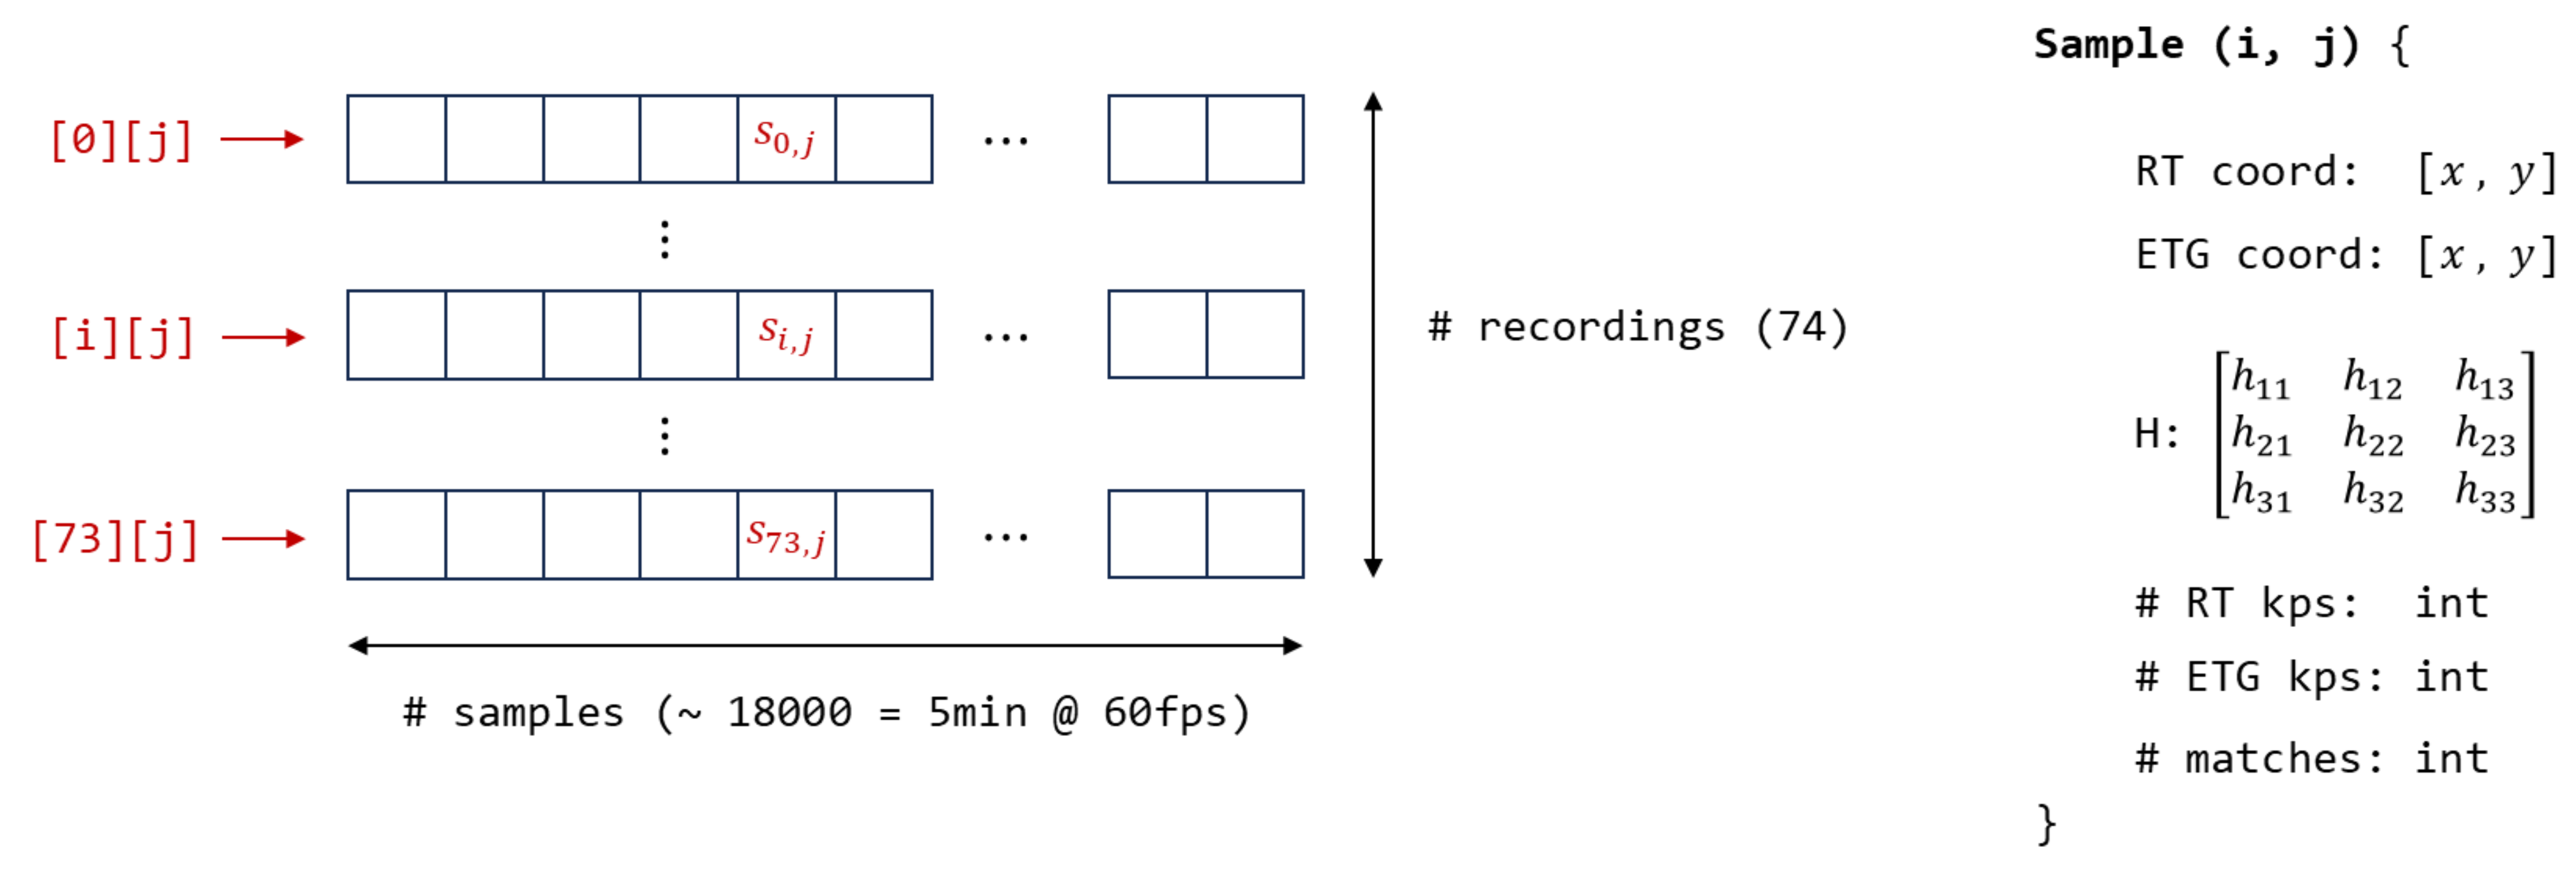
\includegraphics[width=\textwidth]{images/dreyeve/homography_data.png}
    \caption[Data structure to store homographies]
    {The data structure used to store the homographies.
    \textbf{Left}: Each element is a specific sample in the i-th video, at 
    the j-th frame.
    \textbf{Right}: The attributes of each sample.}
    \label{fig:homography_data_structure}
\end{figure}

\subsection{Stereo Camera System Setup}
The cameras recording system can be reconducted to an uncalibrated stereo vision 
setup. In particular, the two cameras are not aligned and the baseline is not 
fixed. However, this is a problem for the projection of 3D world points between 
the two cameras. In fact, homography is a planar transformation, 
and it is possible to estimate the projection matrix if keypoints lie on the 
same plane.
For this reason we decided to make the approximation that the 
keypoints are far away enough from the vehicle. This is a reasonable 
approximation since the driver is usually looking at the road and the objects 
far away from the vehicle. Moreover, the baseline of the stereo vision system is 
small compared to the average depth of the keypoints.

In this way, it is not necessary to know intrinsic and extrinsic parameters of 
the cameras, such as focal length, resolution, and distortion coefficients. 
This approach is also proposed in the Dr(eye)ve paper \cite{dreyeve}.


\subsection{Targets Data Structure}
From the Dr(eye)ve dataset, we extracted the bounding boxes of the vulnerable 
road users, such as pedestrians and cyclists.
Moreover, through ByteTrack \cite{bytetrack}, we tracked the targets to have a 
spatio-temporal representation of the scene. Then, we compare the projected gaze 
of the driver with the location of targets. 

However, it is necessary to consider the quality of the tracking. Even though 
ByteTrack was specifically designed to track also overlapping objects, in driving 
scenarios it is not uncommon to have tracking failures. To partially mitigate 
the problem, we set two different states for each target: a 
\emph{detection} state and an \emph{observation} state.
\begin{itemize}
    \addtolength\itemsep{-2mm}
    \item \textbf{Detection}: the target is being detected and tracked by the algorithms.
    \item \textbf{Observation}: the target is being observed by the driver.
\end{itemize}

\begin{figure}
\centering
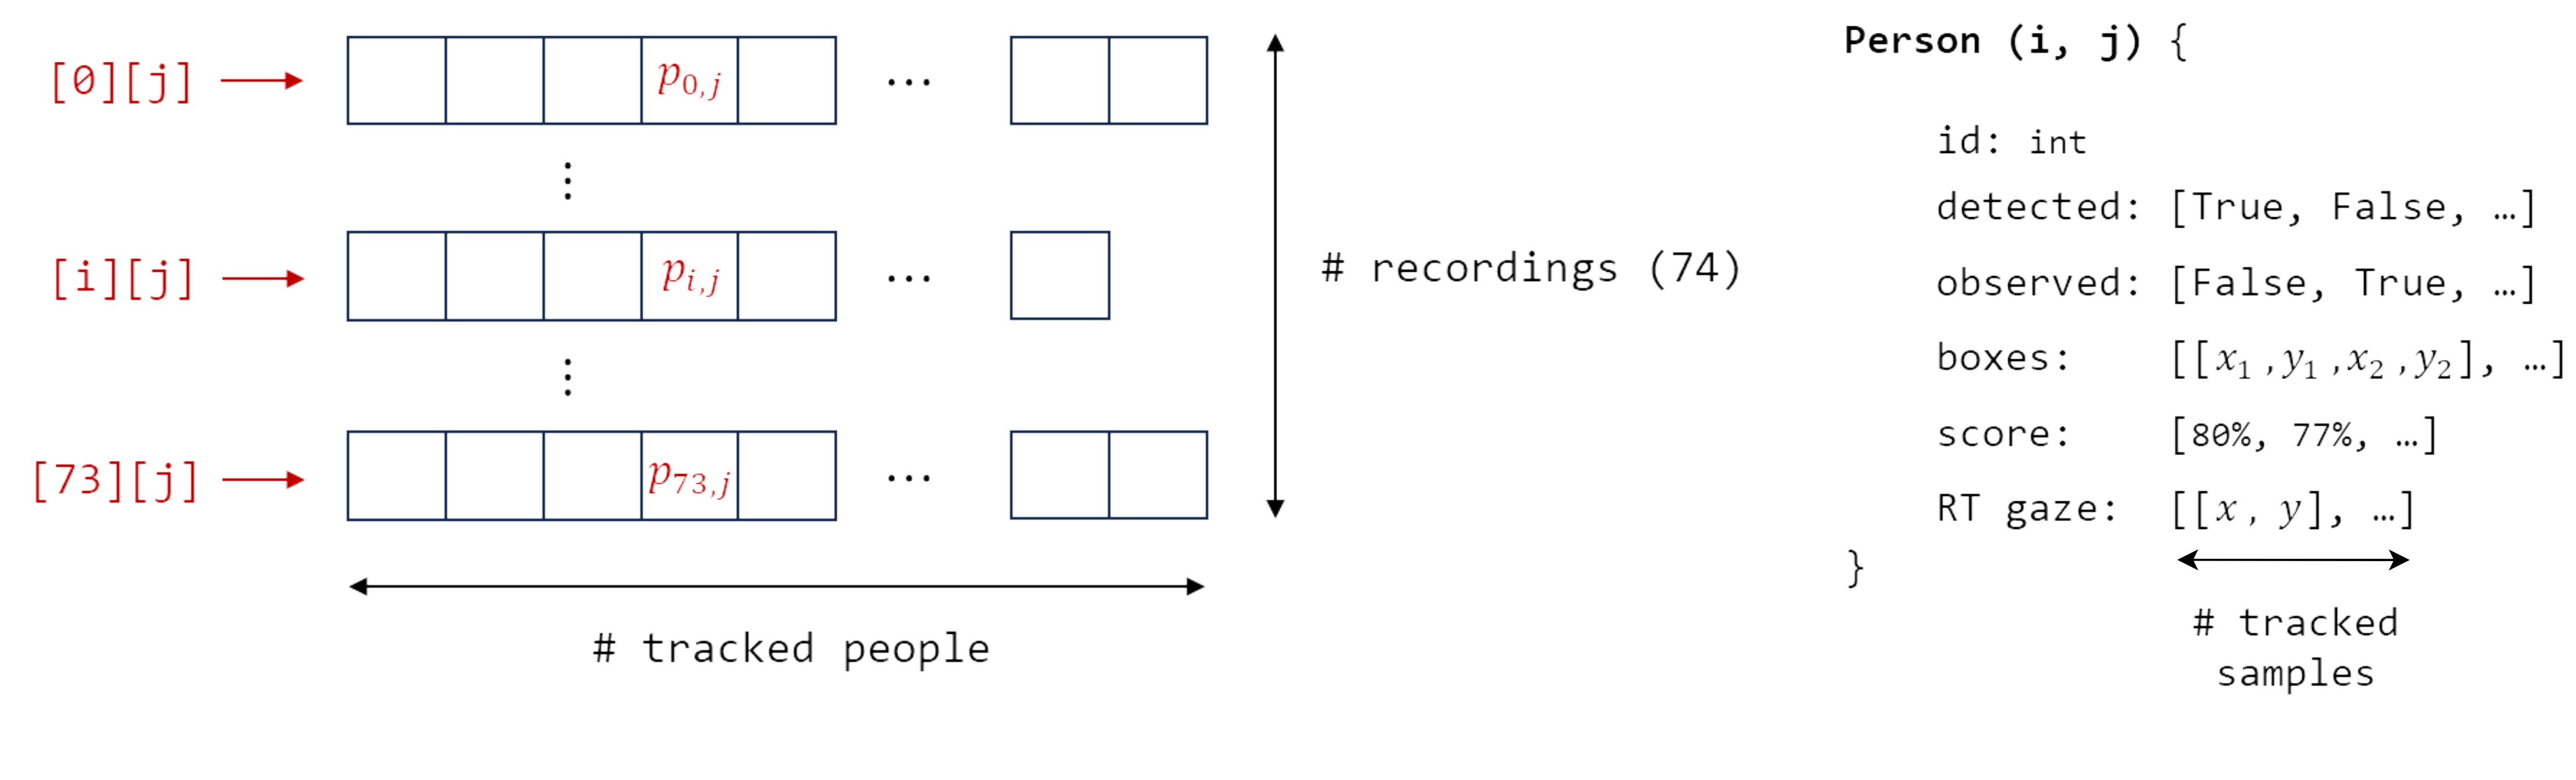
\includegraphics[width=\textwidth]{images/dreyeve/targets_data.png}
\caption[Data structure to store targets' states]
{The data structure used to store targets' states.
\textbf{Left}: Each element is a specific person, which contains the set of 
states during all its tracking.
\textbf{Right}: The attributes of the tracked person during time.
}
\label{fig:targets_data_structure}
\end{figure}
Through this approach, we can make sure if a person is both detected by the 
algorithm and observed by the driver. Without storing the detection data, there 
can be some unclear situations where the driver is looking at a target that is 
partially or completely occluded. That can happen because ByteTrack keeps the 
tracking of occluded targets through a Kalman filter. 
The data structure is represented in details 
in Figure \ref{fig:targets_data_structure}: it is a list of lists where each 
element is a unique person that has been tracked in the respective video.

Each person has the following list of states: a unique tracking ID, the 
detection states, the observation states, the bounding boxes' coordinates with 
the confidence score, and the coordinates of the projected driver's gaze.

\subsection{Adding Depth Information}
Targets' depth information can be very informative for the driver's attention 
model. In fact, the driver is usually more interested in the objects that are 
closer to the vehicle.
Considering the cameras' setup there are three main ways to include depth 
information of the scene: using a neural network to estimate the depth of the 
detected objects from the bounding box dimensions, leveraging the stereo vision 
data and car's location information (GPS and speed) to estimate the depth of 
similar keypoints in consecutive timeframes, or to compute a monocular depth 
map through a pretrained model.

The first approach is the simplest and the fastest, but it is also the less 
accurate. In fact the depth of an object is not only related to its dimensions, 
especially for people. Bounding boxes can vary depending on the target age, pose, 
occlusions and if they are riding a vehicle, like a bicycle. 
Moreover, a custom calibration should be made at least for each camera model, 
with its dedicated lens and image sensor. Image distortion could heavily affect 
the quality of predictions. However, this is not feasible in our case because 
we do not have any ground truth information to fine-tune the model.
Some recent works on targets' depth estimation with stereo vision systems were 
proposed in \cite{li2019stereo}, \cite{Peng_2020_CVPR}. There are also studies 
on retrieving the depth of objects from monocular images \cite{bbox_mde}.

The second approach is the most accurate and robust, but it requires an accurate 
calibration of the stereo vision system to perform well. Moreover, data depth 
is only related to correspondent keypoints. This means that if no matching 
keypoints related to a target are found, it is not possible to estimate its 
depth. Finally, the stereo vision system is not always reliable, especially when 
it is uncalibrated and the baseline is not fixed and relatively small compared to 
the average depth of the keypoints. 
Recently some self-calibration methods have been proposed 
\cite{sfm_self_calibration1}, \cite{sfm_self_calibration2}.
The roof top camera has a wide field of 
view because it uses a wide angle lens, and then an anti-distortion algorithm 
is computed. This affects the quality of the depth estimation.

The third approach is the most versatile and suitable to the specific application.
In fact, the dense depth map computed by the pretrained model is not related to the 
ETG camera and allows to estimate the depth of all the objects in the scene.
The model is trained on a large dataset and is able to generalize well to 
different scenarios. The only drawback is that the depth map is not absolute. 
This means that it is not possible to estimate the distance of objects in meters, 
but through a relative scale depending on the maximum and minimum depths of the 
scene. However, this should not be able to compromise the quality of the 
driver's attention model because that is the same approach we use as humans 
when driving. However, we actually compute a hybrid approach where we use a sort 
of stereo vision system through our eyes and our knowledge and past experience 
to make an approximate estimation of the depth of the objects.
In the experiments section we will show the performance of pretrained MiDaS 
\cite{midas}.

\begin{figure}
\centering
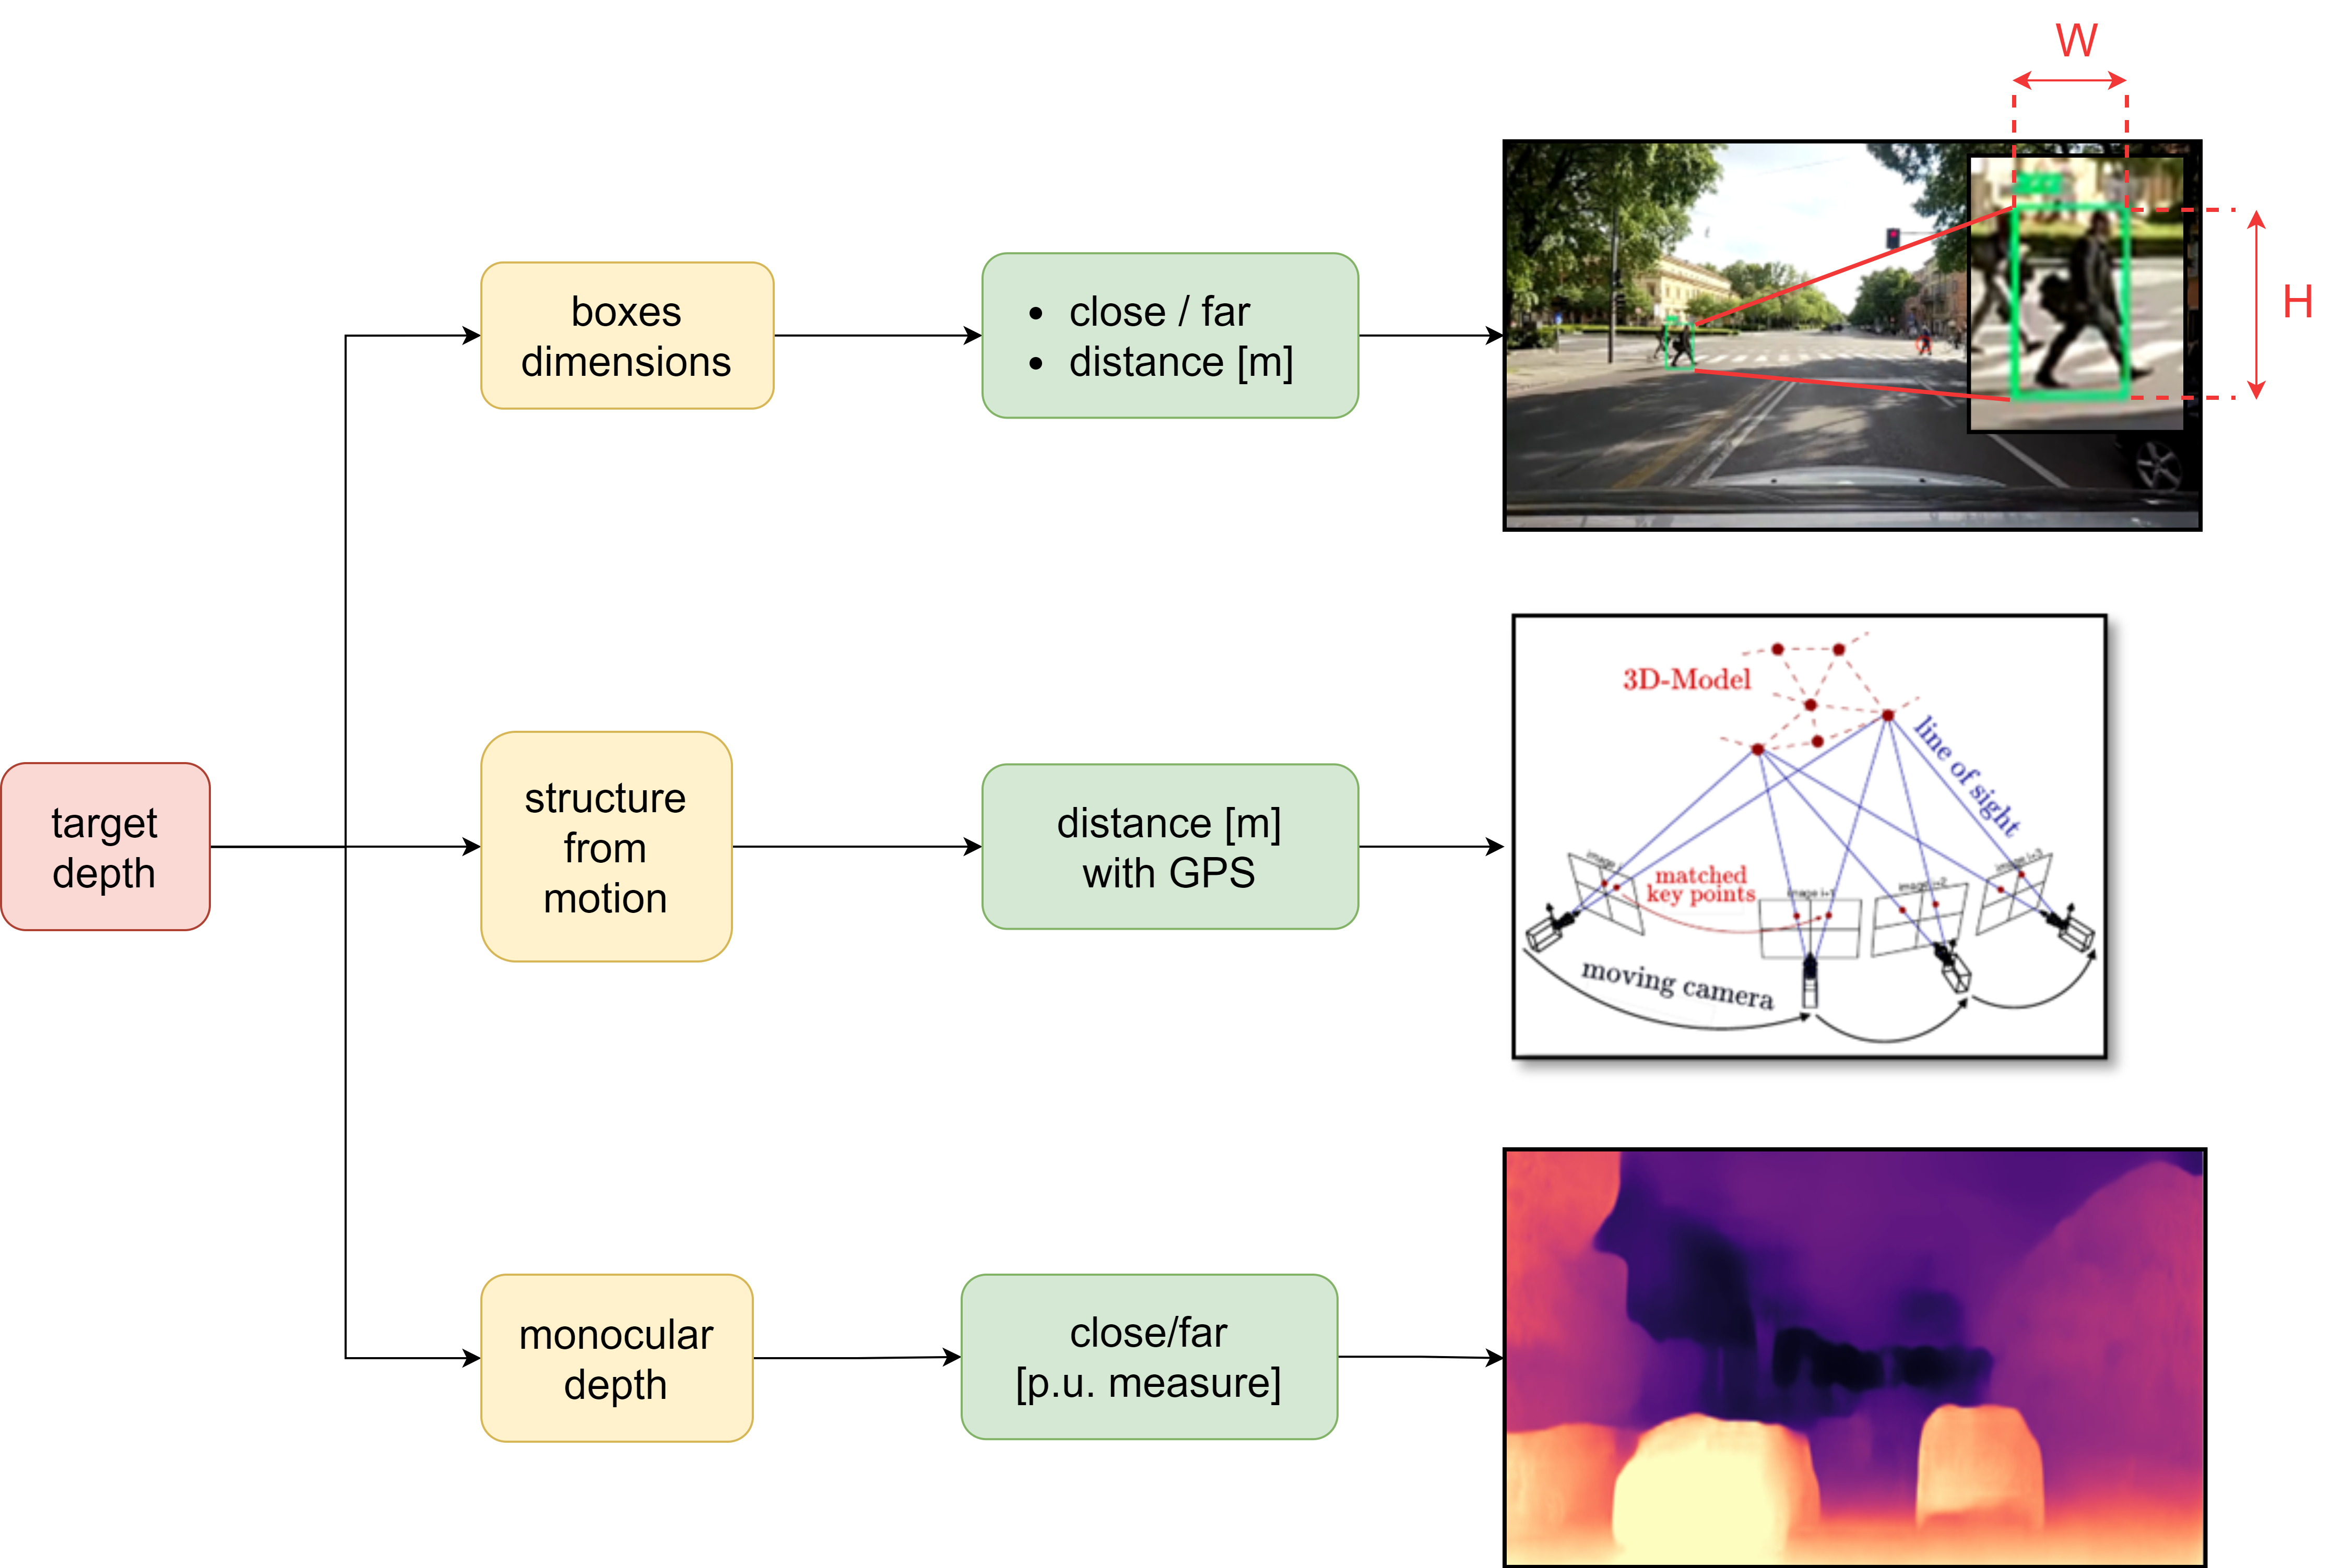
\includegraphics[width=\textwidth]{images/dreyeve/depth_estimation.png}
\caption[Three possible methods to estimate targets' depth]
{Summary of the possible three methods to estimate the depth of targets.}
\label{fig:depth_estimation}
\end{figure}



\subsection{Adding Spatial Information}
Spatial information can be fundamental to analyze the driver's attention 
towards targets in the scene. In fact, the driver usually pays more attention 
to some locations of the field of view, depending on the context (e.g. type of 
road, traffic, weather conditions, crowdness, etc.).
Moreover, the double camera setup allows to have a wider field of view on the 
rooftop camera. This is particularly useful to track the gaze also when the 
driver is moving the head. 

Therefore, an initial approach is to include the spatial information of the 
gaze in the driver's attention model. In particular, we divided the roof top 
camera view in a 3x7 grid, as shown in Figure \ref{fig:rt_camera_grid}. 
This division is made to have a more detailed representation of the scene, in 
fact it is possible to notice that cells from  1 to 7 are out of interest when 
the driver is looking straight ahead. These area are 
located on the top of the image, where the driver is usually not looking at, 
except for some specific situations (e.g. traffic lights, road signs, etc.). 

Cells 8, 9, 13, 14 represent out of field of view areas, where there could be 
potential threats (e.g. a pedestrian crossing the road from the left side, 
a car crossing the road). 

Cells 10, 11, 12 are the center of the field of view, 
where the driver is usually looking at. In particular, considering the city 
center shown in Figure \ref{fig:rt_camera_grid}, area 11 captures front 
vehicles. 
Cells 10, 12, show possible targets interacting 
in the near future with the ego-vehicle 
from the road sides (e.g. the ego-vehicle approaching a crosswalk with a 
pedestrian waiting to cross the road).

Cells 15, 16, 20, 21 represent the left and sie corners out of the field of view 
of the ETG camera. These areas are similar to cells 8, 9, 13, 14, but on with 
closer targets. Therefore they are more dangerous because targets on these 
locations are more challenging to spot and the driver has less time to react.

Cell 17, 18, 19 are at the bottom-center of the field of view.
These areas cover in part the dashboard of the car, and the driver is usually 
looking at them when checking the speed, the fuel, the GPS, etc. 
Depending on the context, these areas could also cover close vehicles on the 
front of the ego-vehicle (e.g. a line of vehicles at a traffic light). 
Therefore, these areas can identify a warning when the driver is not 
looking at the road and there is a potential threat.

In general, we identified different areas of interest in the field of view of 
the driver, depending on the specific context. This is an initial equal division 
that still helps characterize the scene. However, considering the wide view of 
the roof top camera, and the distortion applied to the image, there are better 
solutions to divide the scene. For example, it is possible to make a non-equal 
division, grouping together areas that are more similar to each other.
In summary, spatial information is both informative and complicated to manage 
because it is highly dependent on the context. Therefore, it could be helpful 
to let a model learn the spatial information by itself, through a deep learning 
approach. This mainly motivates the move from the traditional computer 
vision-based approach to the deep learning-based approach.
 
\begin{figure}
\centering
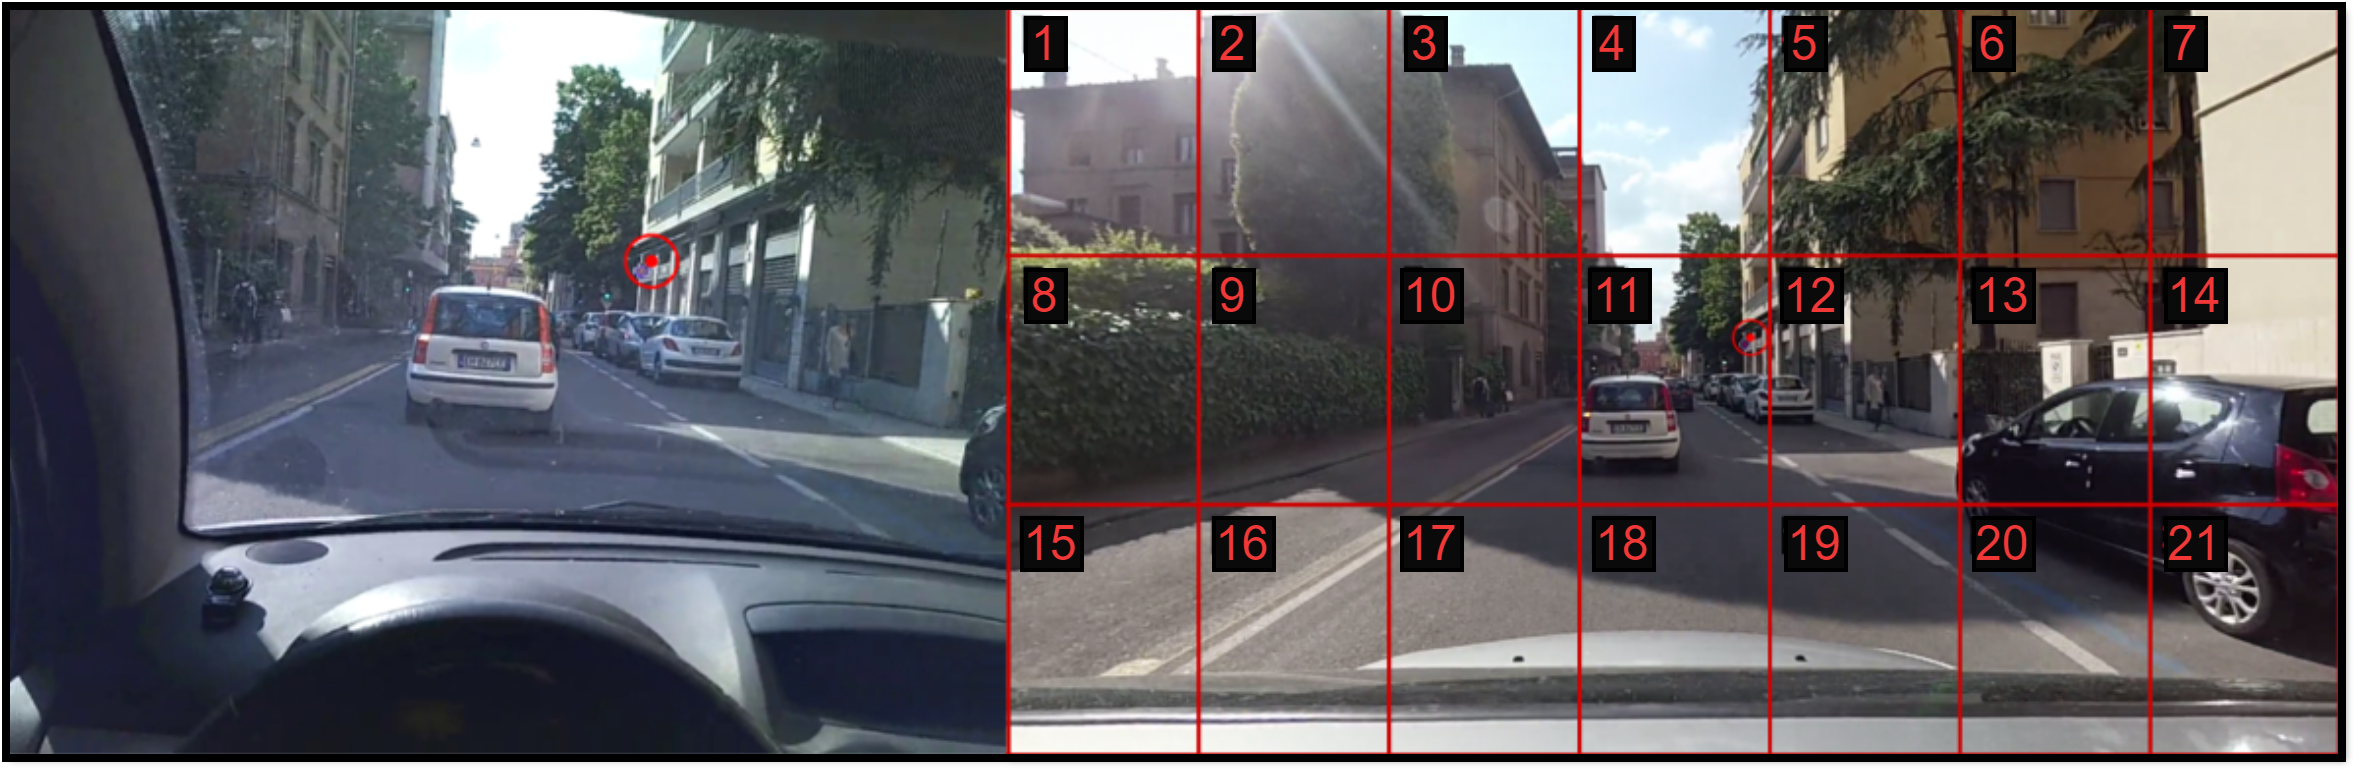
\includegraphics[width=\textwidth]{images/dreyeve/rt_cam_grid.png}
\caption[Grid division of the roof top camera view]
{Division of the roof top camera view in a 3x7 grid.}
\label{fig:rt_camera_grid}
\end{figure}


\section{Deep Learning-based Approach}
In this section we describe the deep learning-based approach to the driver's 
attention model.
Even though in the previous section we identified the main stages of the 
traditional computer vision-based approach, and many positive aspects were 
highlighted, there are also some drawbacks.
In particular, for each stage there are some simplification hypothesis that 
affect quality of inputs for the driver's attention model.

For example, the homography projection of the gaze is not perfect, and the 
approximation that the matched keypoints are far away enough from the vehicle 
is not always true. Moreover, the quality of homography estimation heavily 
depends on the quality of the keypoints' detection and matching. This can be 
compromised by the quality of the images, presence of occlusions, light and 
weather conditions, etc.

The scene perception stage is also affected by the quality of the detection 
and tracking algorithms. In particular, ByteTrack is not always able to track
overlapping objects, and the quality of the tracking is affected by the 
quality of the detection. Moreover, the detection is not always perfect, and 
there are some false positives and false negatives. 

Depth estimation stage is also affected by the quality of the pretrained 
model of MiDaS. In particular, the model is trained on a large datasets in 
completely different contexts, and it is not always able to generalize well to 
different scenarios. Moreover, the depth map is not absolute, and it is not 
possible to estimate the absoulte distance in meters.

That is why it is better to let a model learn important features automatically, through 
some classification biases used to label a dataset. We decided to use a vision 
transformer model to learn the self-attention map of the scene to detect 
potential threats.
Four main experiments were made: supervised and semi-supervised training on Dr(eye)ve, 
supervised and semi-supervised training on BDD100k.
The general scheme is shown in Figure \ref{fig:dl_approach_scheme}; as it is 
possible to notice, the scheme does not consists of some blocks to extract 
indirect features from the scene, but it is mainly focused on the deep learning 
model to learn the features by itself by camera images. In particular, the 
attention model is represented by two vision transformers: one is the teacher and 
the other is the student. The teacher is in charge of generating pseudo labels 
for the student from the unlabelled dataset. The trained student is then used 
to make the final predictions, and it is supposed to perform better than the
teacher.
\begin{figure}
\centering
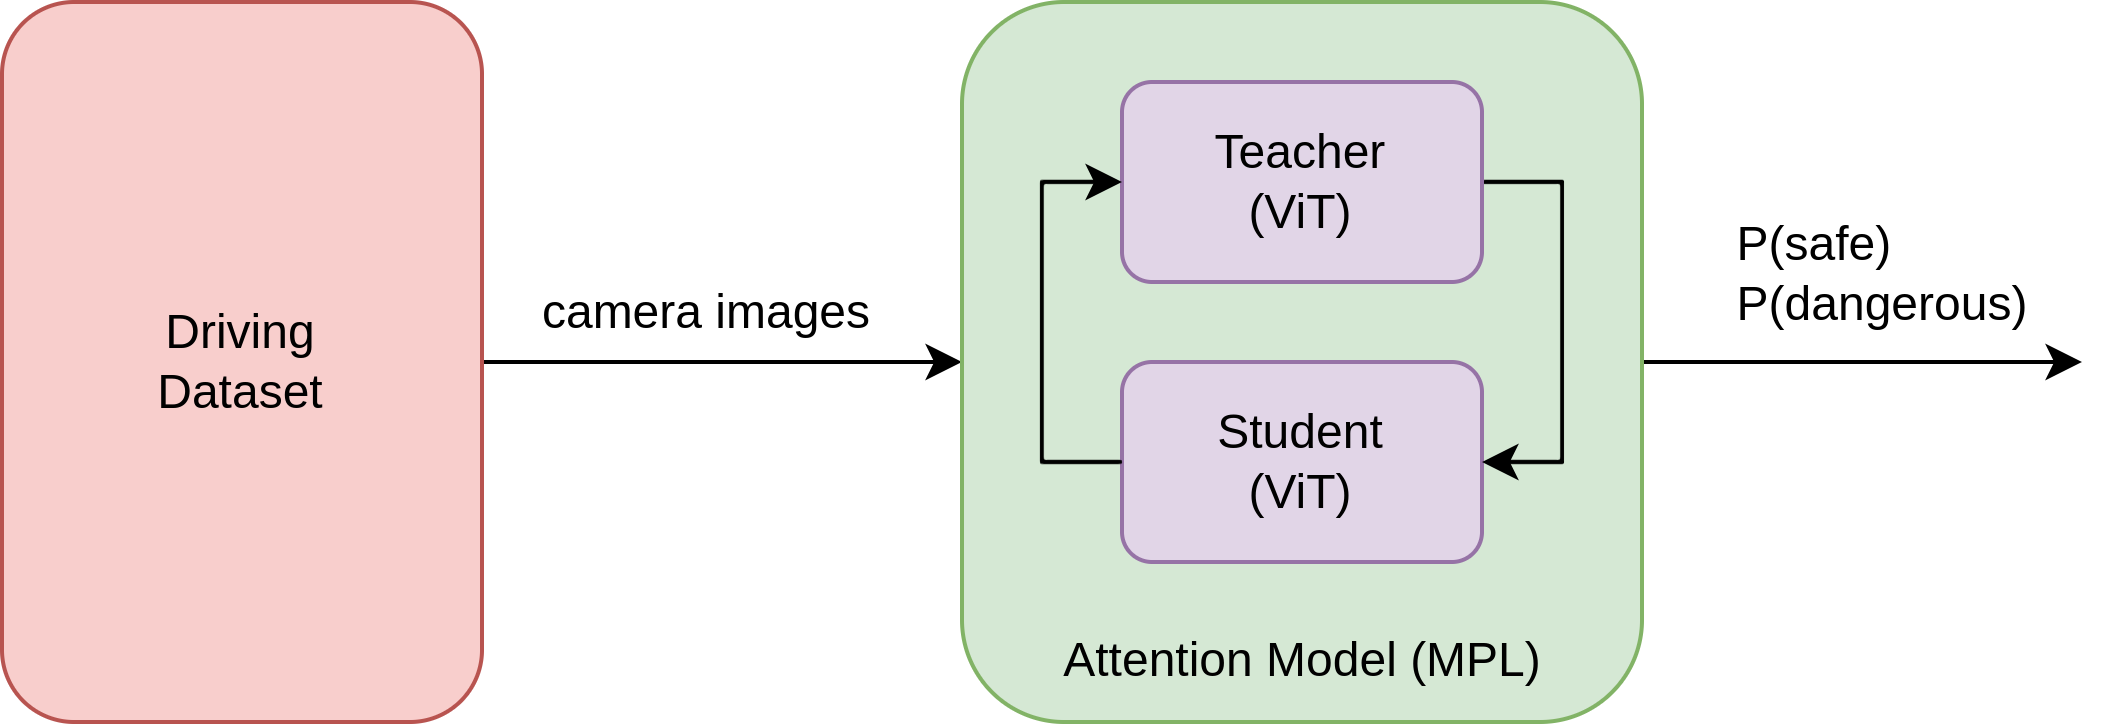
\includegraphics[width=0.85\textwidth]{images/ssl/dl_approach_scheme.png}
\vspace{0.4cm}
\caption[Deep learning-based detection model of dangerous scenarios.]
{General scheme of the deep learning-based approach for detecting
dangerous situations in driving scenarios.}
\label{fig:dl_approach_scheme}
\end{figure}

\subsection{Attention Map for Anomaly Detection}
The vision transformer model is able to learn an attention map of the scene for 
each head. This feature is useful to let the model learn many spatial relations 
between patches. The idea is to have many images labeled by humans to detect 
dangerous situations in a driving dataset. Then, we can use the attention map 
to spot critical areas of the scene that are more likely to be related to 
dangerous situations.
It is also possible to check if attention maps are consistent with the human 
decision bias with a test set.

An example of attention maps for a pre-trained multi-head vision transformer is 
shown in Figure \ref{fig:attention_maps}.
It is possible to notice that each head is focusing on some areas of the 
scene, learning different relations. This is particularly useful to detect 
anomalies in the scene, such as a pedestrian crossing the road, a car approaching 
the ego-vehicle, etc. In this particular case, the model is pre-trained on 
ImageNet, therefore many highlighted areas correspond to the presence of 
people and cars. However, in the fifht head the model extracts more general 
features to combine with the desired targets.

\subsubsection{Artificial Bias}
Labelling an entire dataset with dangerous situations is a very challenging 
task. On one hand, it is not always possible to have a clear definition of what 
is a dangerous situation. In fact, it is highly dependent on the context, the 
person who is labelling and the driving experience. On the other hand, it is 
very time consuming and expensive to label a large dataset.

Therefore, we decided to start using an \emph{artificial bias} to classify 
dangerous situations. In particular, we used two different criterias to label 
Dr(eye)ve and BDD100k datasets. In Dr(eye)ve, we used the following criteria:
a driving scene is considered dangerous if there is at least one vulnerable 
road user (e.g. pedestrian, cyclist) or one car; the scene is condidered safe 
otherwise.

In BDD100k, on the other hand, we used the following criteria: a driving scene 
is considered dangerous if there is at least one vulnerable user (e.g. pedestrian, 
cyclist) or a bicycle; the scene is considered safe otherwise.

The main motivation for the change from Dr(eye)ve to BDD100k is that the former 
dataset does not have any human annotations regarding location of targets. 
Therefore an object detector was used to accomplish the task. However, the 
quality of the detection is not always perfect, and there are some false 
positives and false negatives.
The latter, on the other hand, has high-quality human annotations for many 
classes. Moreover, it is the largest dataset available for driving scenarios, 
because each labelled frame corresponds to the frame at the tenth second of 
a driving video. This is particularly useful to leverage semi-supervised learning 
techniques, like Meta Pseudo Labels \cite{pham2021meta}.

Finally, we used two different labelling rules and two different datasets because 
Dr(eye)ve has many more frames with no other vehicles in the scene (recordings 
during night, in the countryside, etc.), while BDD100k has a high percentage of 
frames containing other vehicles. Therefore, the second labelling method is to 
have a less skewed dataset.
However, the two methods should not affect the model training, since we are 
grouping frames according to the presence of some objects, that the model should 
find out from the training set.
%
\newlength{\subfigwidth}
\setlength{\subfigwidth}{32mm}
\newlength{\horspace}
\setlength{\horspace}{.25\textwidth}
\begin{figure}
    \caption[Attention maps for a pre-trained multi-head ViT.]
    {Attention masks for a pre-trained multi-head ViT \cite{attention_vit}.}
    \centering
    \begin{tabular}{r p{\horspace} p{\horspace} p{\horspace}}
    Original & 
    \begin{subfigure}[b]{\subfigwidth}
        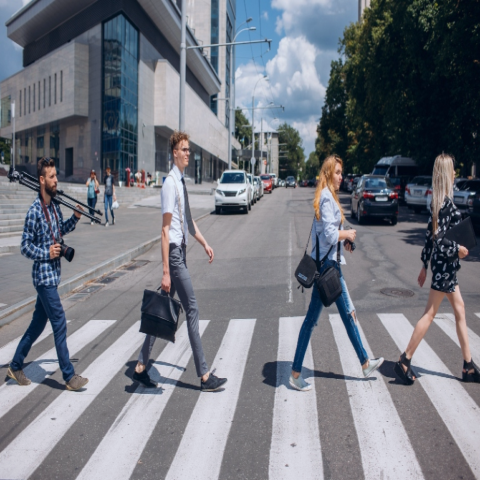
\includegraphics[width=\subfigwidth]{images/vit_attention/1/img.png}
    \end{subfigure}
    \hfill &
    \begin{subfigure}[b]{\subfigwidth}
        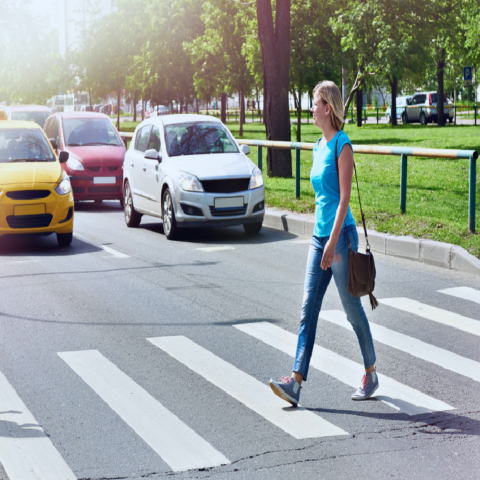
\includegraphics[width=\subfigwidth]{images/vit_attention/2/img.png}
    \end{subfigure} 
    \hfill &
    \begin{subfigure}[b]{\subfigwidth}
        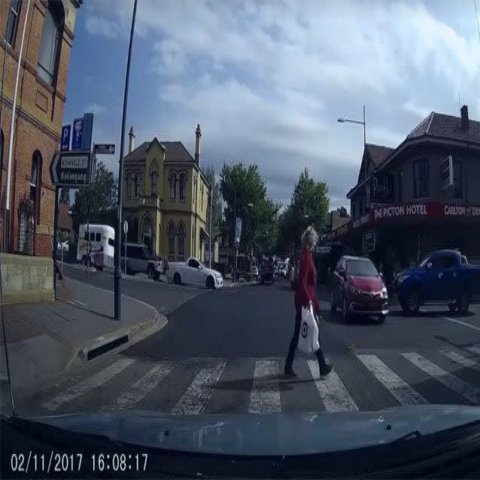
\includegraphics[width=\subfigwidth]{images/vit_attention/4/img.png}
    \end{subfigure} \\
    %
    Head 1 &
    \begin{subfigure}[b]{\subfigwidth}
        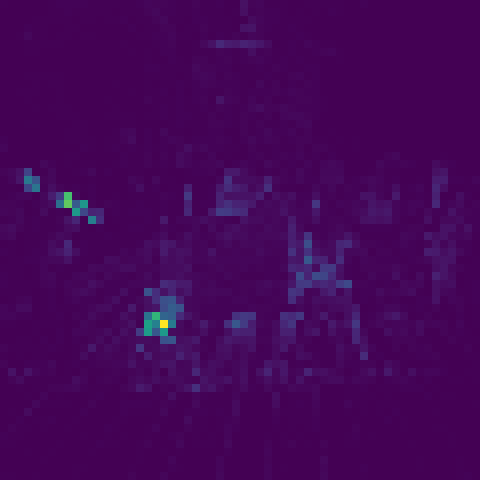
\includegraphics[width=\subfigwidth]{images/vit_attention/1/attn-head0.png}
    \end{subfigure}
    \hfill &
    \begin{subfigure}[b]{\subfigwidth}
        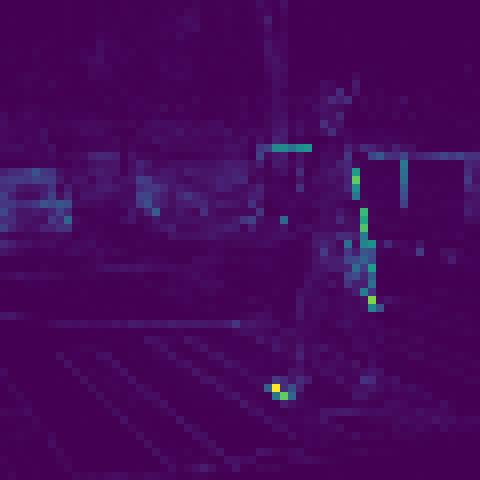
\includegraphics[width=\subfigwidth]{images/vit_attention/2/attn-head0.png}
    \end{subfigure} 
    \hfill &
    \begin{subfigure}[b]{\subfigwidth}
        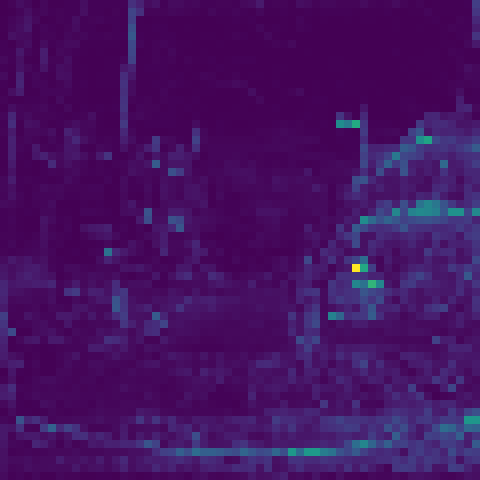
\includegraphics[width=\subfigwidth]{images/vit_attention/4/attn-head0.png}
    \end{subfigure} \\
    %
    Head 2 &
    \begin{subfigure}[b]{\subfigwidth}
        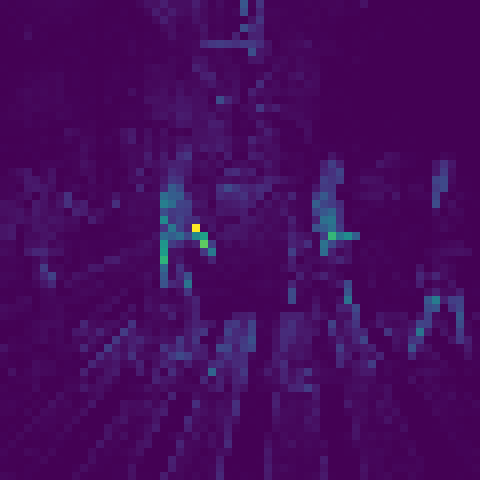
\includegraphics[width=\subfigwidth]{images/vit_attention/1/attn-head1.png}
    \end{subfigure}
    \hfill &
    \begin{subfigure}[b]{\subfigwidth}
        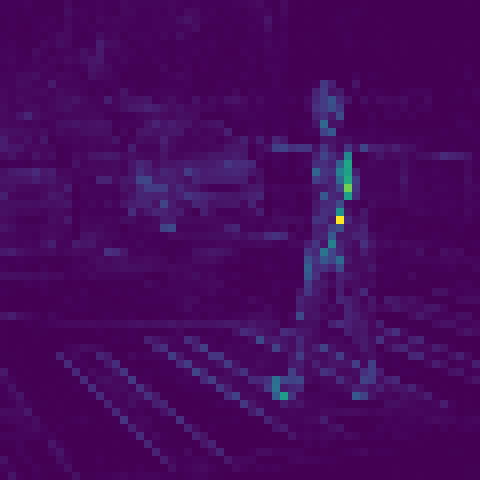
\includegraphics[width=\subfigwidth]{images/vit_attention/2/attn-head1.png}
    \end{subfigure} 
    \hfill &
    \begin{subfigure}[b]{\subfigwidth}
        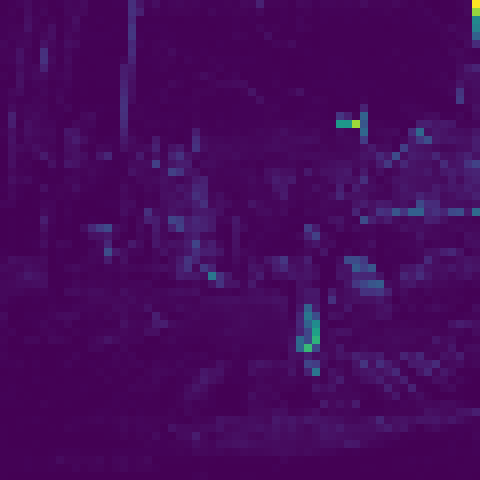
\includegraphics[width=\subfigwidth]{images/vit_attention/4/attn-head1.png}
    \end{subfigure} \\
    Head 3 &
    \begin{subfigure}[b]{\subfigwidth}
        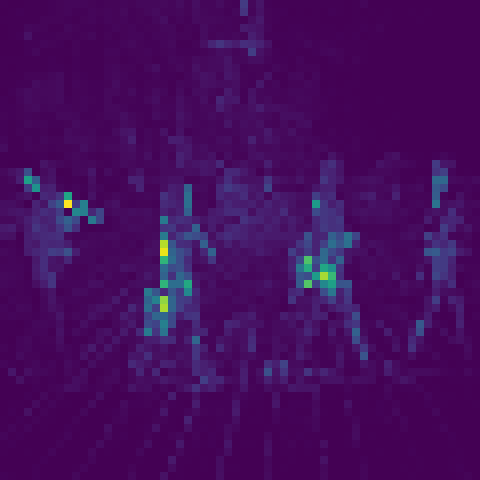
\includegraphics[width=\subfigwidth]{images/vit_attention/1/attn-head2.png}
    \end{subfigure}
    \hfill &
    \begin{subfigure}[b]{\subfigwidth}
        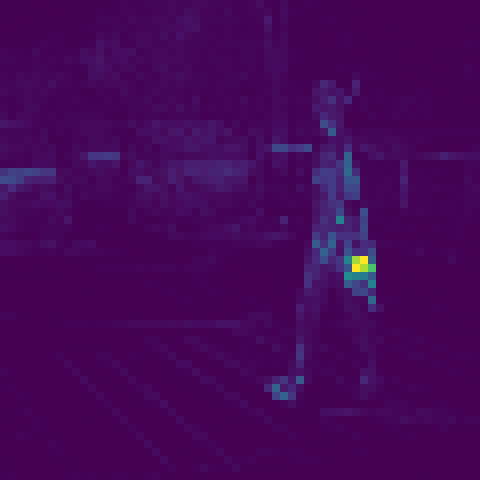
\includegraphics[width=\subfigwidth]{images/vit_attention/2/attn-head2.png}
    \end{subfigure} 
    \hfill &
    \begin{subfigure}[b]{\subfigwidth}
        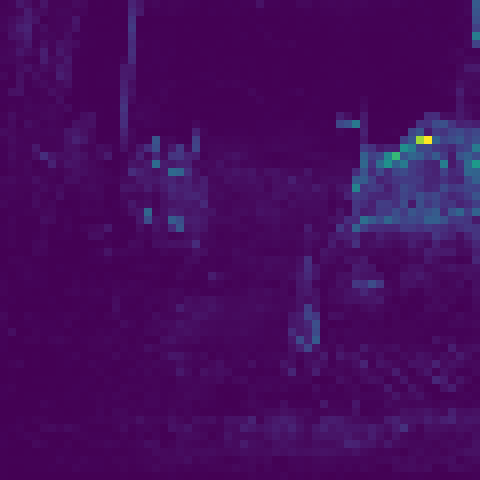
\includegraphics[width=\subfigwidth]{images/vit_attention/4/attn-head2.png}
    \end{subfigure} \\
    Head 4 &
    \begin{subfigure}[b]{\subfigwidth}
        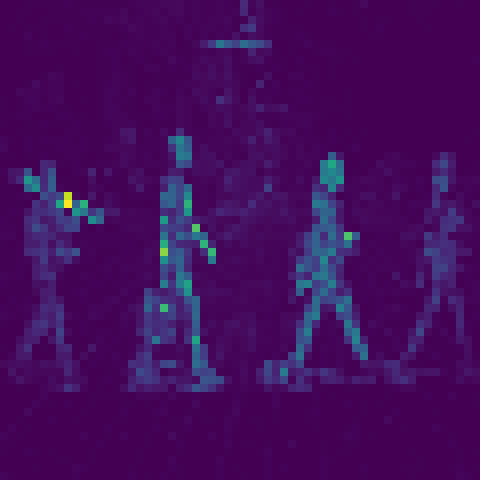
\includegraphics[width=\subfigwidth]{images/vit_attention/1/attn-head3.png}
    \end{subfigure}
    \hfill &
    \begin{subfigure}[b]{\subfigwidth}
        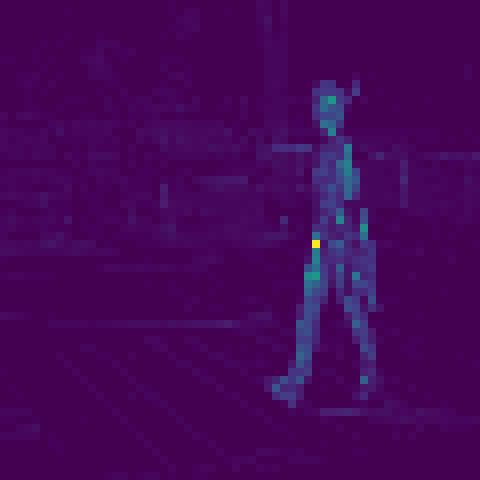
\includegraphics[width=\subfigwidth]{images/vit_attention/2/attn-head3.png}
    \end{subfigure} 
    \hfill &
    \begin{subfigure}[b]{\subfigwidth}
        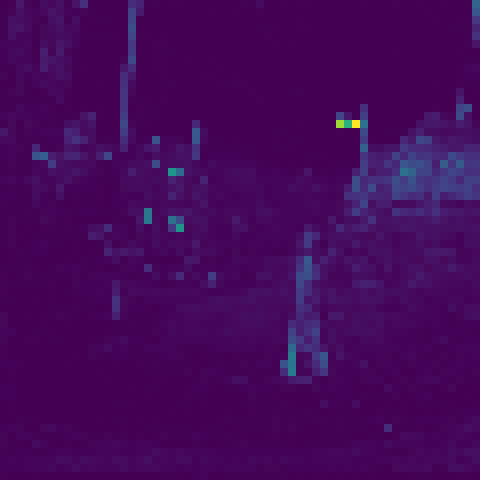
\includegraphics[width=\subfigwidth]{images/vit_attention/4/attn-head3.png}
    \end{subfigure} \\
    Head 5 &
    \begin{subfigure}[b]{\subfigwidth}
        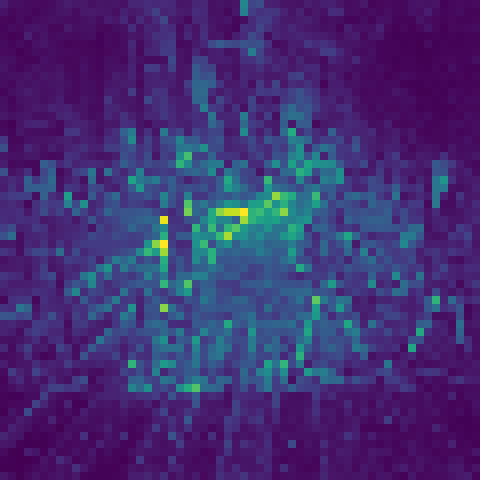
\includegraphics[width=\subfigwidth]{images/vit_attention/1/attn-head4.png}
    \end{subfigure}
    \hfill &
    \begin{subfigure}[b]{\subfigwidth}
        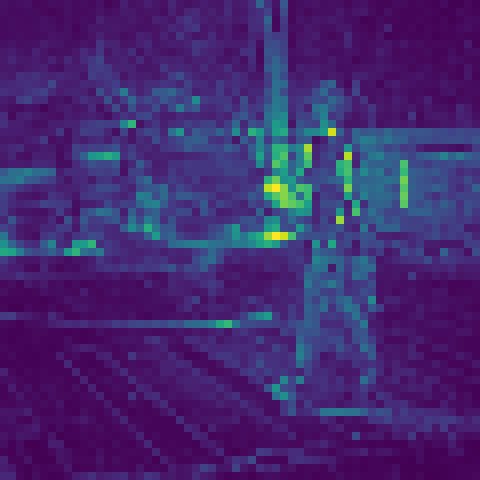
\includegraphics[width=\subfigwidth]{images/vit_attention/2/attn-head4.png}
    \end{subfigure} 
    \hfill &
    \begin{subfigure}[b]{\subfigwidth}
        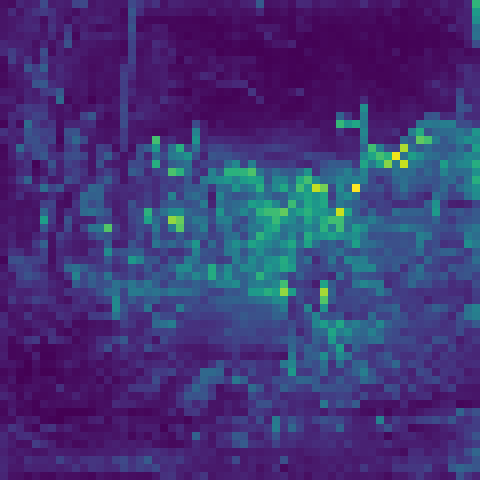
\includegraphics[width=\subfigwidth]{images/vit_attention/4/attn-head4.png}
    \end{subfigure} \\
    Head 6 &
    \begin{subfigure}[b]{\subfigwidth}
        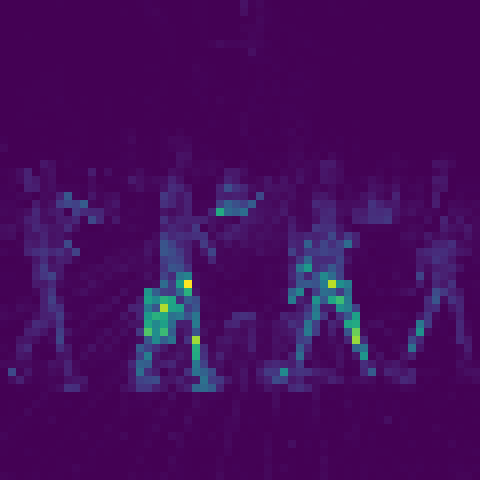
\includegraphics[width=\subfigwidth]{images/vit_attention/1/attn-head5.png}
    \end{subfigure}
    \hfill &
    \begin{subfigure}[b]{\subfigwidth}
        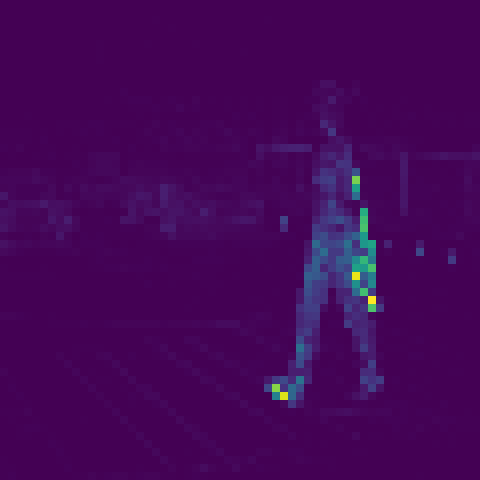
\includegraphics[width=\subfigwidth]{images/vit_attention/2/attn-head5.png}
    \end{subfigure} 
    \hfill &
    \begin{subfigure}[b]{\subfigwidth}
        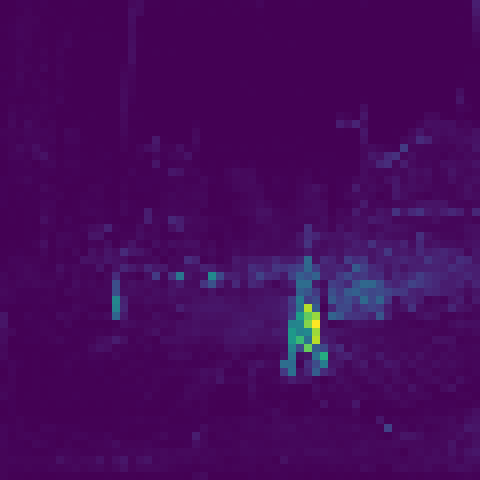
\includegraphics[width=\subfigwidth]{images/vit_attention/4/attn-head5.png}
    \end{subfigure} \\
\label{fig:attention_maps}
\end{tabular}
\end{figure}

\subsection{Data Preprocessing of Dr(eye)ve}
The Dr(eye)ve dataset is composed of 74 video sequences of five minutes each.
To reduce redundancy of images it was downsampled at 4 fps and resized and 
stretched to 300x300 pixels. Then RetinaNet \cite{retinanet} was used to detect 
the desired targets, 
and the label was assigned to the frame if at least one of the targets was detected.

Then we divided the dataset in training, validation and test sets. In particular,
the validation set is based on 1000 images, 
equally balanced between dangerous and safe situations.
The test set is based on 200 images, also equally balanced between dangerous 
and safe cases.
Both the validation and test sets are always kept fixed, with the same ratio.

On the other hand, the training set has different sizes, because we made some 
experiments in both supervised and semi-supervised learning, changing the 
labelled training size to figure out how it affected the predictions.
Therefore, we started with 500 labels, then 1000, 2500, 5000 and 10000.
The initial training set is not equally distributed between dangerous and safe 
cases (around 63\% of safe cases and 37\% of dangerous cases).
A further training set with 40000 labels was also made to better understand the 
model's behavior with a large amount of labelled data.

\subsection{Training Pipeline on Dr(eye)ve}
Starting from the smallest training set, when increasing labels after each 
experiment, we still use RetinaNet to classify new images. However, the criteria 
to augment the training set is based on the model's predictions. In particular, 
we used the object detector as a \emph{validator} to correct wrong predictions.
In summary, the training pipeline can be described in the following way:
%
\begin{enumerate}
    \addtolength\itemsep{-2mm}
    \item Prepare training, validation and test sets.
    \item Train the model and stop when reaching maximum validation accuracy.
    \item Pick new samples from the unlabeled set and predict the labels.
    \item Use RetinaNet to determine ground-truth labels on the picked samples.
    \item Update the training set with wrong samples.
    \item Go to point 2.
\end{enumerate}
In particular, when increasing the training set, we compensate the unbalance 
between dangerous and safe cases by picking the same number of wrong predictions 
between the two classes. This is particularly useful to avoid the model to 
overfit on the majority class.
However, we also weight the loss function to give more importance to the 
minority class.

The same pipeline is used for training models with Meta Pseudo Labels, but in 
this case the unlabeled set is both used to train the model and to pick new 
samples to label. Moreover, we stopped the training when reaching the maximum 
validation accuracy of the student. 

\subsection{Data Preprocessing of BDD100k}
The BDD100K dataset is a large and diverse driving video database designed for 
the development and evaluation of automated driving technologies. It includes 
100,000 videos captured from various geographic, environmental, and weather 
conditions.
Each video in the BDD100K dataset is typically about 40 seconds long, recorded 
at 30 frames per second, resulting in approximately 1,200 frames per video. 
However, only 100,000 frames are completely labelled by humans, and each frame 
corresponds to the tenth second of a video.

Therefore, we used all the labelled frames and downsampled the unlabeled set (the 
videos) at 3fps. This is to reduce redundancy of data in semi-supervised 
learning and speeding-up the training process.
We also resized and stretched all frames to 600x600 pixels. We chose this 
resolution because it is a good trade-off between details of the scene and 
computational cost.

In this case it not required to use any validator because we only used 
human-labelled frames for the labelled training set. In particular, we labelled 
a frame as dangerous if there is at least one vulnerable target, including 
pedestrians, riders, bicycles. The scene is considered safe otherwise.
However, considering the trade-off between resolution and details described above, 
we choose to set a minimum threshold of the area occupied by the bounding box 
of the target to consider the scene as dangerous. This is particularly useful 
to have more reliable data, to make sure that the model is able to extract 
enough useful feature from.
The minimum threshold area is set to 5000 pixels for each target in the original 
image resolution of 1280x720 pixels.

\subsection{Handling Unbalanced Data}
Managing unbalanced datasets in binary classification poses significant challenges 
due to the disproportionate distribution of the classes. In such scenarios, 
models trained on these datasets might exhibit a bias toward the majority class, 
often at the expense of the minority class. This can lead to a situation where 
the model performs well statistically in terms of overall accuracy but fails to 
correctly identify instances of the less frequent class.

The complexity arises because the usual evaluation metric, accuracy, does not 
reflect the model's performance on the minority class effectively. 
This misrepresentation can lead to misleading conclusions about the model's true 
effectiveness, especially in the BDD100k dataset, where there is a proportion 
of 90\% of safe cases and 10\% of dangerous cases.

To address these challenges, it's crucial to employ a suite of metrics that 
provide a more comprehensive view of the model’s performance across both classes. 
Metrics such as precision, recall, F1-score, and others allow for a more detailed 
assessment of how well the model identifies and classifies instances from both the 
majority and minority classes. Each metric highlights different aspects of the 
model's behavior, such as its ability to correctly predict positive cases, avoid 
false positives, or balance these factors through a combined score. 
By considering these metrics, we can better understand 
and mitigate the biases inherent in models trained on unbalanced datasets.

\subsubsection{Evaluation Metrics}
In the context of unbalanced datasets like Dr(eye)ve and BDD100k, traditional 
accuracy, which simply measures the proportion of total correct predictions 
relative to the total dataset size, can be misleading. For instance, in BDD100k 
dataset, where 90\% of the data are of one class, a naive model predicting only 
that class would achieve 90\% accuracy, despite not having learned to identify 
the rarer class effectively.

Instead, more nuanced metrics such as precision, recall, and F1-score are used. 
Precision is the ratio of correctly predicted positive observations to the total 
predicted positives. It is defined as:
\begin{equation*}
    \text{Precision} = \frac{TP}{TP + FP}
\end{equation*}
where TP is the number of true positives and FP is the number of false positives. 
This metric helps to understand the accuracy of the positive predictions.

Recall (or sensitivity) measures the ability of a model to find all the relevant 
cases within a dataset. It is calculated by:
\begin{equation*}
    \text{Recall} = \text{Sensitivity} = \frac{TP}{TP + FN}
\end{equation*}
where FN is the number of false negatives. This metric is crucial for cases where 
missing a positive instance is significantly worse than falsely labeling negative 
instances as positive.

The F1-score is the harmonic mean of precision and recall, and is calculated by:
\begin{equation*}
    \text{F1-score} = 2 \times \frac{\text{Precision} \times \text{Recall}}{\text{Precision} + \text{Recall}}
\end{equation*}
This score is particularly useful for unbalanced datasets because it takes both 
false positives and false negatives into account, providing a more realistic 
measure of a model’s performance, especially when the classes are unevenly 
distributed.

In case of Dr(eye)ve this problem does not affect the validation set because it 
is forced to be balanced. However, the training set is unbalanced, and the model 
could overfit on the majority class, even though we also weighted the loss 
function. In this case, we used the F1-score as the main metric to evaluate the 
model's performance.

In case of BDD100k, on the other hand, the problem affects both the training 
and validation sets. In this case, we used the F1-score as the main metric to 
evaluate the model's performance. However, we also considered recall as an 
important metric to evaluate the model's ability to find all the relevant cases 
within the dataset, even though it could lead to more false positives.

\subsubsection{Receiver Operating Characteristic (ROC) Curve}
The Receiver Operating Characteristic (ROC) curve is a crucial tool for 
evaluating binary classification models, particularly in scenarios like detecting 
dangerous scenes in driving datasets, where the data is highly unbalanced. 
The ROC curve plots the true positive rate (sensitivity) against the false positive 
rate (1 - specificity) at various threshold settings. 
Sensitivity, as described above is also called recall, and specificity is 
defined as the true negative rate, or the proportion of negative instances 
correctly identified as such:
\begin{equation*}
    \text{Specificity} = \frac{TN}{TN + FP}
\end{equation*}


\begin{figure}
    \centering
    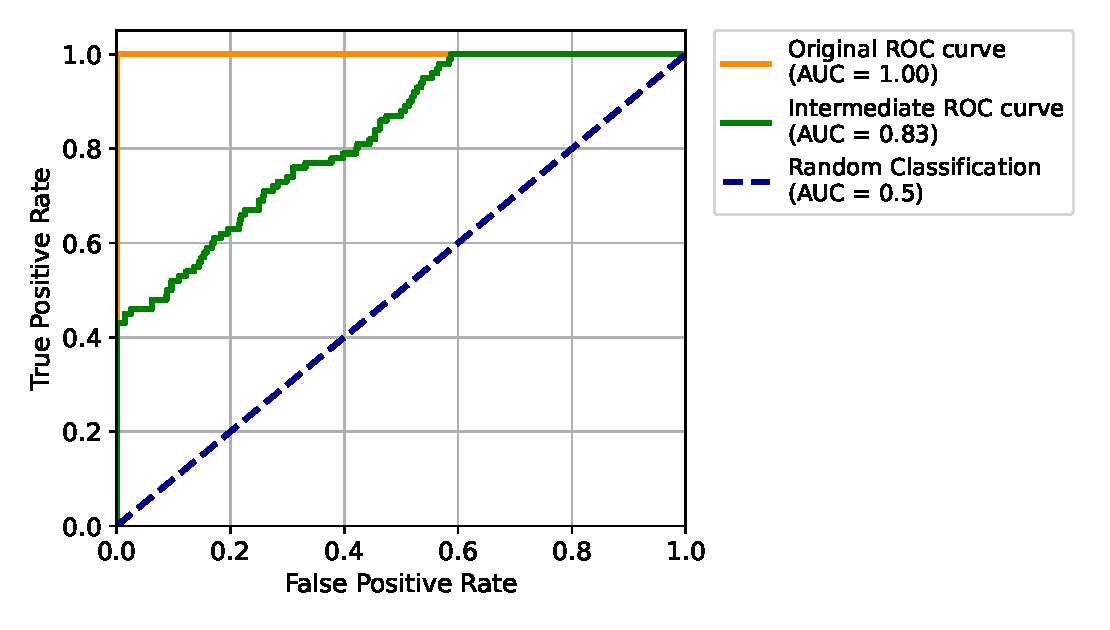
\includegraphics[width=0.95\textwidth]{images/roc/roc_curve.pdf}
    \caption
    {Example of ROC curve for a binary classification model.}
    \label{fig:roc_curve}
\end{figure}
This curve helps to 
visualize the trade-off between sensitivity and specificity from the two extreme 
operation points (with a threshold of 0.0 and 1.0).
In fact, it is possible to notice that setting a threshold of 0.0, the model 
will output all positive cases, then the sensitivity will be 1.0, but the 
specificity will be 0.0. On the other hand, setting a threshold of 1.0, the model 
will output all negative cases, then the specificity will be 1.0, but the 
sensitivity will be 0.0. An example of ROC curve is shown in Figure 
\ref{fig:roc_curve}.

Setting the operation point on the ROC curve involves choosing a specific 
threshold that defines how the binary classifier will categorize positive and 
negative classes. This threshold setting is crucial in unbalanced datasets 
because it helps balance the sensitivity and specificity according to the 
specific needs of the application. For instance, in detecting dangerous driving 
scenes, missing a dangerous scene (low sensitivity) might be more critical than 
incorrectly labeling a safe scene as dangerous (high specificity). Therefore, 
we choose a threshold that prioritizes sensitivity.

The optimal solution often depends on the specific costs associated with false 
positives and false negatives. These can be explicitly defined through a cost 
function, which quantifies the impact of these errors. For instance, a cost 
function could be constructed such that the cost of missing a dangerous scene 
(false negative) is set higher than incorrectly identifying a scene as dangerous 
(false positive). By minimizing this cost function across possible thresholds, 
we can determine the most cost-effective operation point on the ROC curve.